\chapter{Architecture}

	\section{Diagramme de classes}
	\subsection{Diagramme de Packages}
		\begin{figure}[h!]
	   	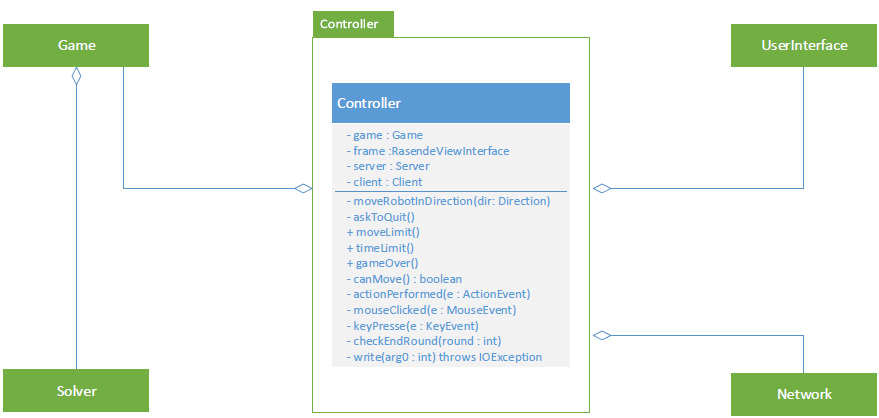
\includegraphics[scale=0.6]{img/packages.png}
		\end{figure}
\newpage
	\subsection{Package Game}
		\begin{figure}[h!]
	   	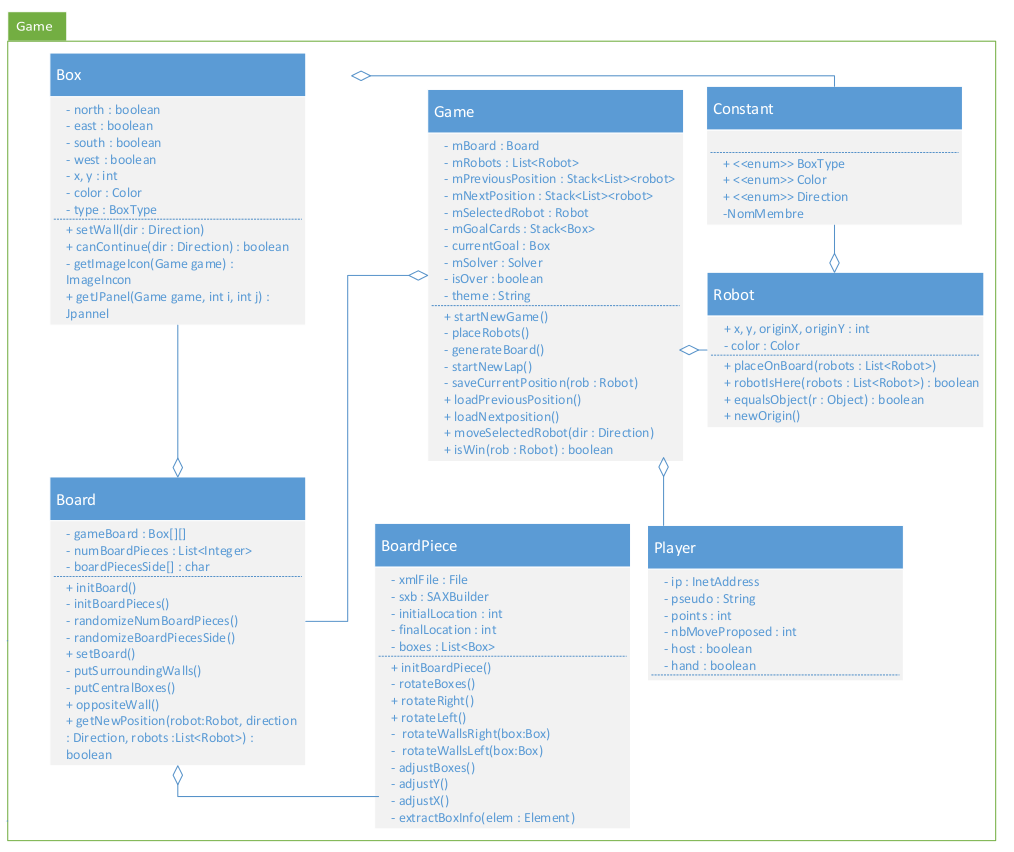
\includegraphics[scale=0.6]{img/game.png}
		\end{figure}
\newpage
	\subsection{Package Network}
		\begin{figure}[h!]
	   	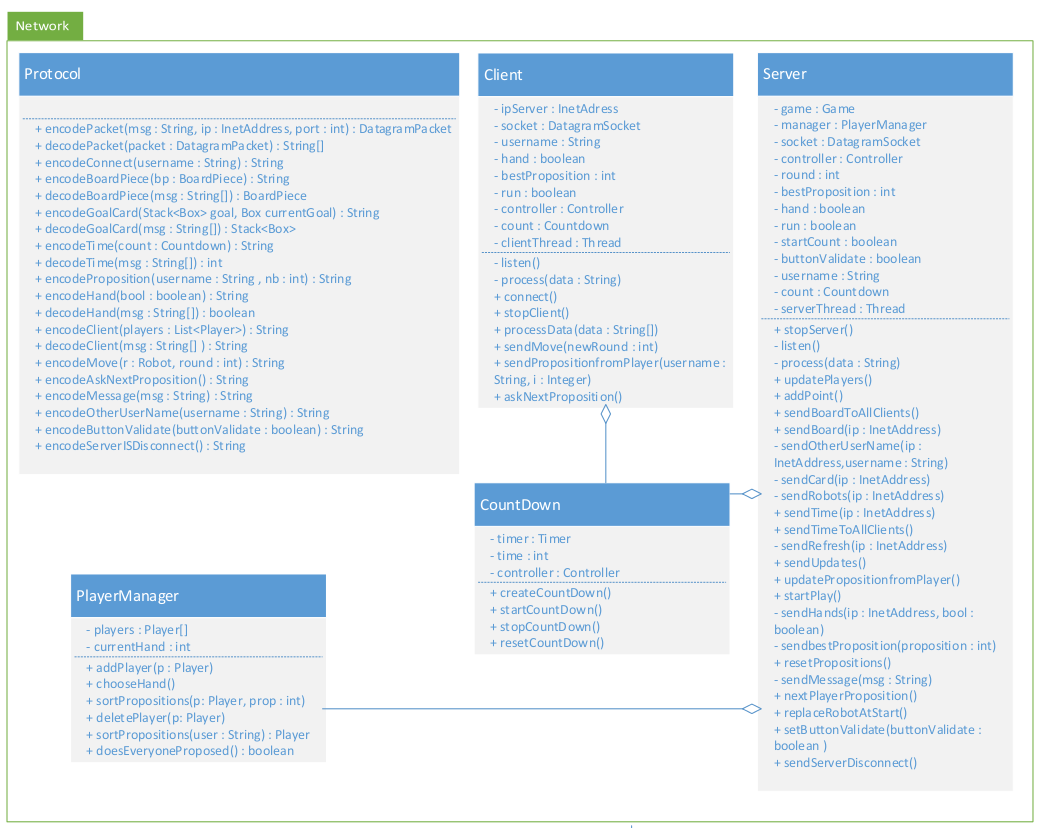
\includegraphics[scale=0.6]{img/network.png}
		\end{figure}
\newpage
	\subsection{Package UserInterface}
		\begin{figure}[h!]
	   	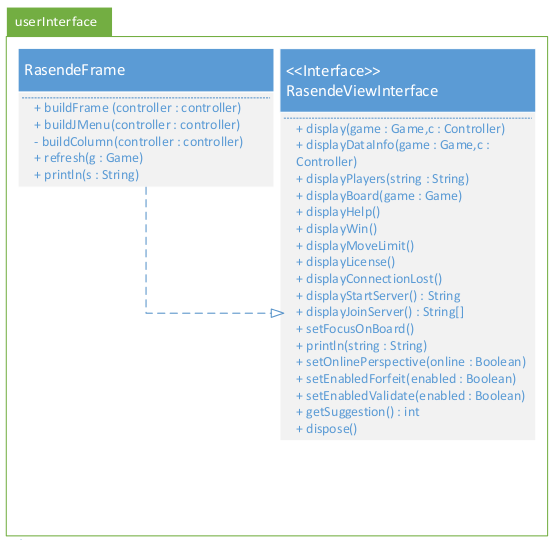
\includegraphics[scale=0.7]{img/userinterface.png}
		\end{figure}
\newpage
	\subsection{Package Solver}
		\begin{figure}[h!]
	   	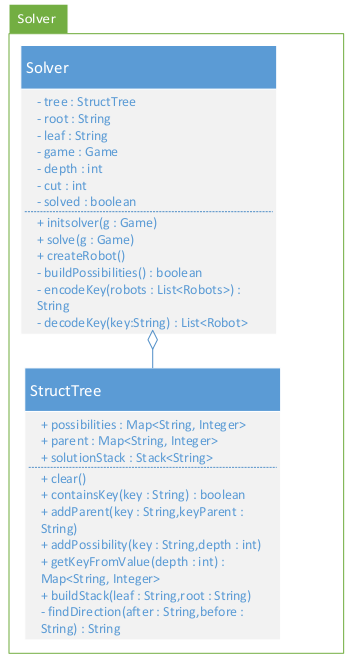
\includegraphics[scale=0.7]{img/solver.png}
		\end{figure}
\newpage
		
	\section{Explications détaillés}
	
	\subsection{MVC}
	
	Nous avons choisi d'utiliser l'architecture Modèle-Vue-Contrôleur pour notre projet de programmation. Notre projet s'organise en plusieurs packages qui représentent les différentes composantes de l'architecture MVC.\\
	
\begin{enumerate}

\item[-]Le package Game correspond à notre modèle. Il contient tous les éléments qui constituent le jeu, comme par exemple les robots ou encore le plateau. 
\item[-]Le package Network contient le code relatif au réseau.
\item[-]Le package Solver contient le code relatif à l'algorithme de résolution de la partie.
\item[-]Le package UserInterface contient la classe qui nous servira à générer une interface graphique. 
\item[-]Dans le package Controller, nous trouvons la classe Controller qui nous servira à faire le lien entre le modèle et la vue. 
\item[-]Le package Main contient la classe Main qui servira au lancement de notre logiciel.
\item[-]Le package Test contiendra les différentes classes où sont effectués les test. Ce package n'a pas d'influence sur notre architecture.

\end{enumerate}

	Le package Game contient les classes Board et BoardPiece qui servent à instancier le plateau de jeu grâce à des fichiers xml. La création des plateaux de jeu est expliquée dans une autre partie de ce rapport. 
	
	La classe Box contient les informations relatives à une case du plateau. C'est à dire si elle contient un symbole objectif, ou encore si elle contient un mur. 
	
	La classe Constant répertorie toutes le constantes que nous utilisons, comme par exemple les couleurs des robots, ou bien les directions possibles pour le déplacement des robots.
	
	 La classe Player contient les informations relatives à un joueur. Cette classe est utilisée dans la partie réseau, elle nous permet d'assigner une adresse ip, ou encore un pseudo à un joueur. 
	 
	 La classe Robot sert à instancier les pions du jeu. 
	 
	 Enfin la classe Game regroupe tous les éléments présentés ci-dessus, elle représente notre modèle.
	 
	 


	Voici un schéma pour montrer comment s'articule notre architecture MVC :
	
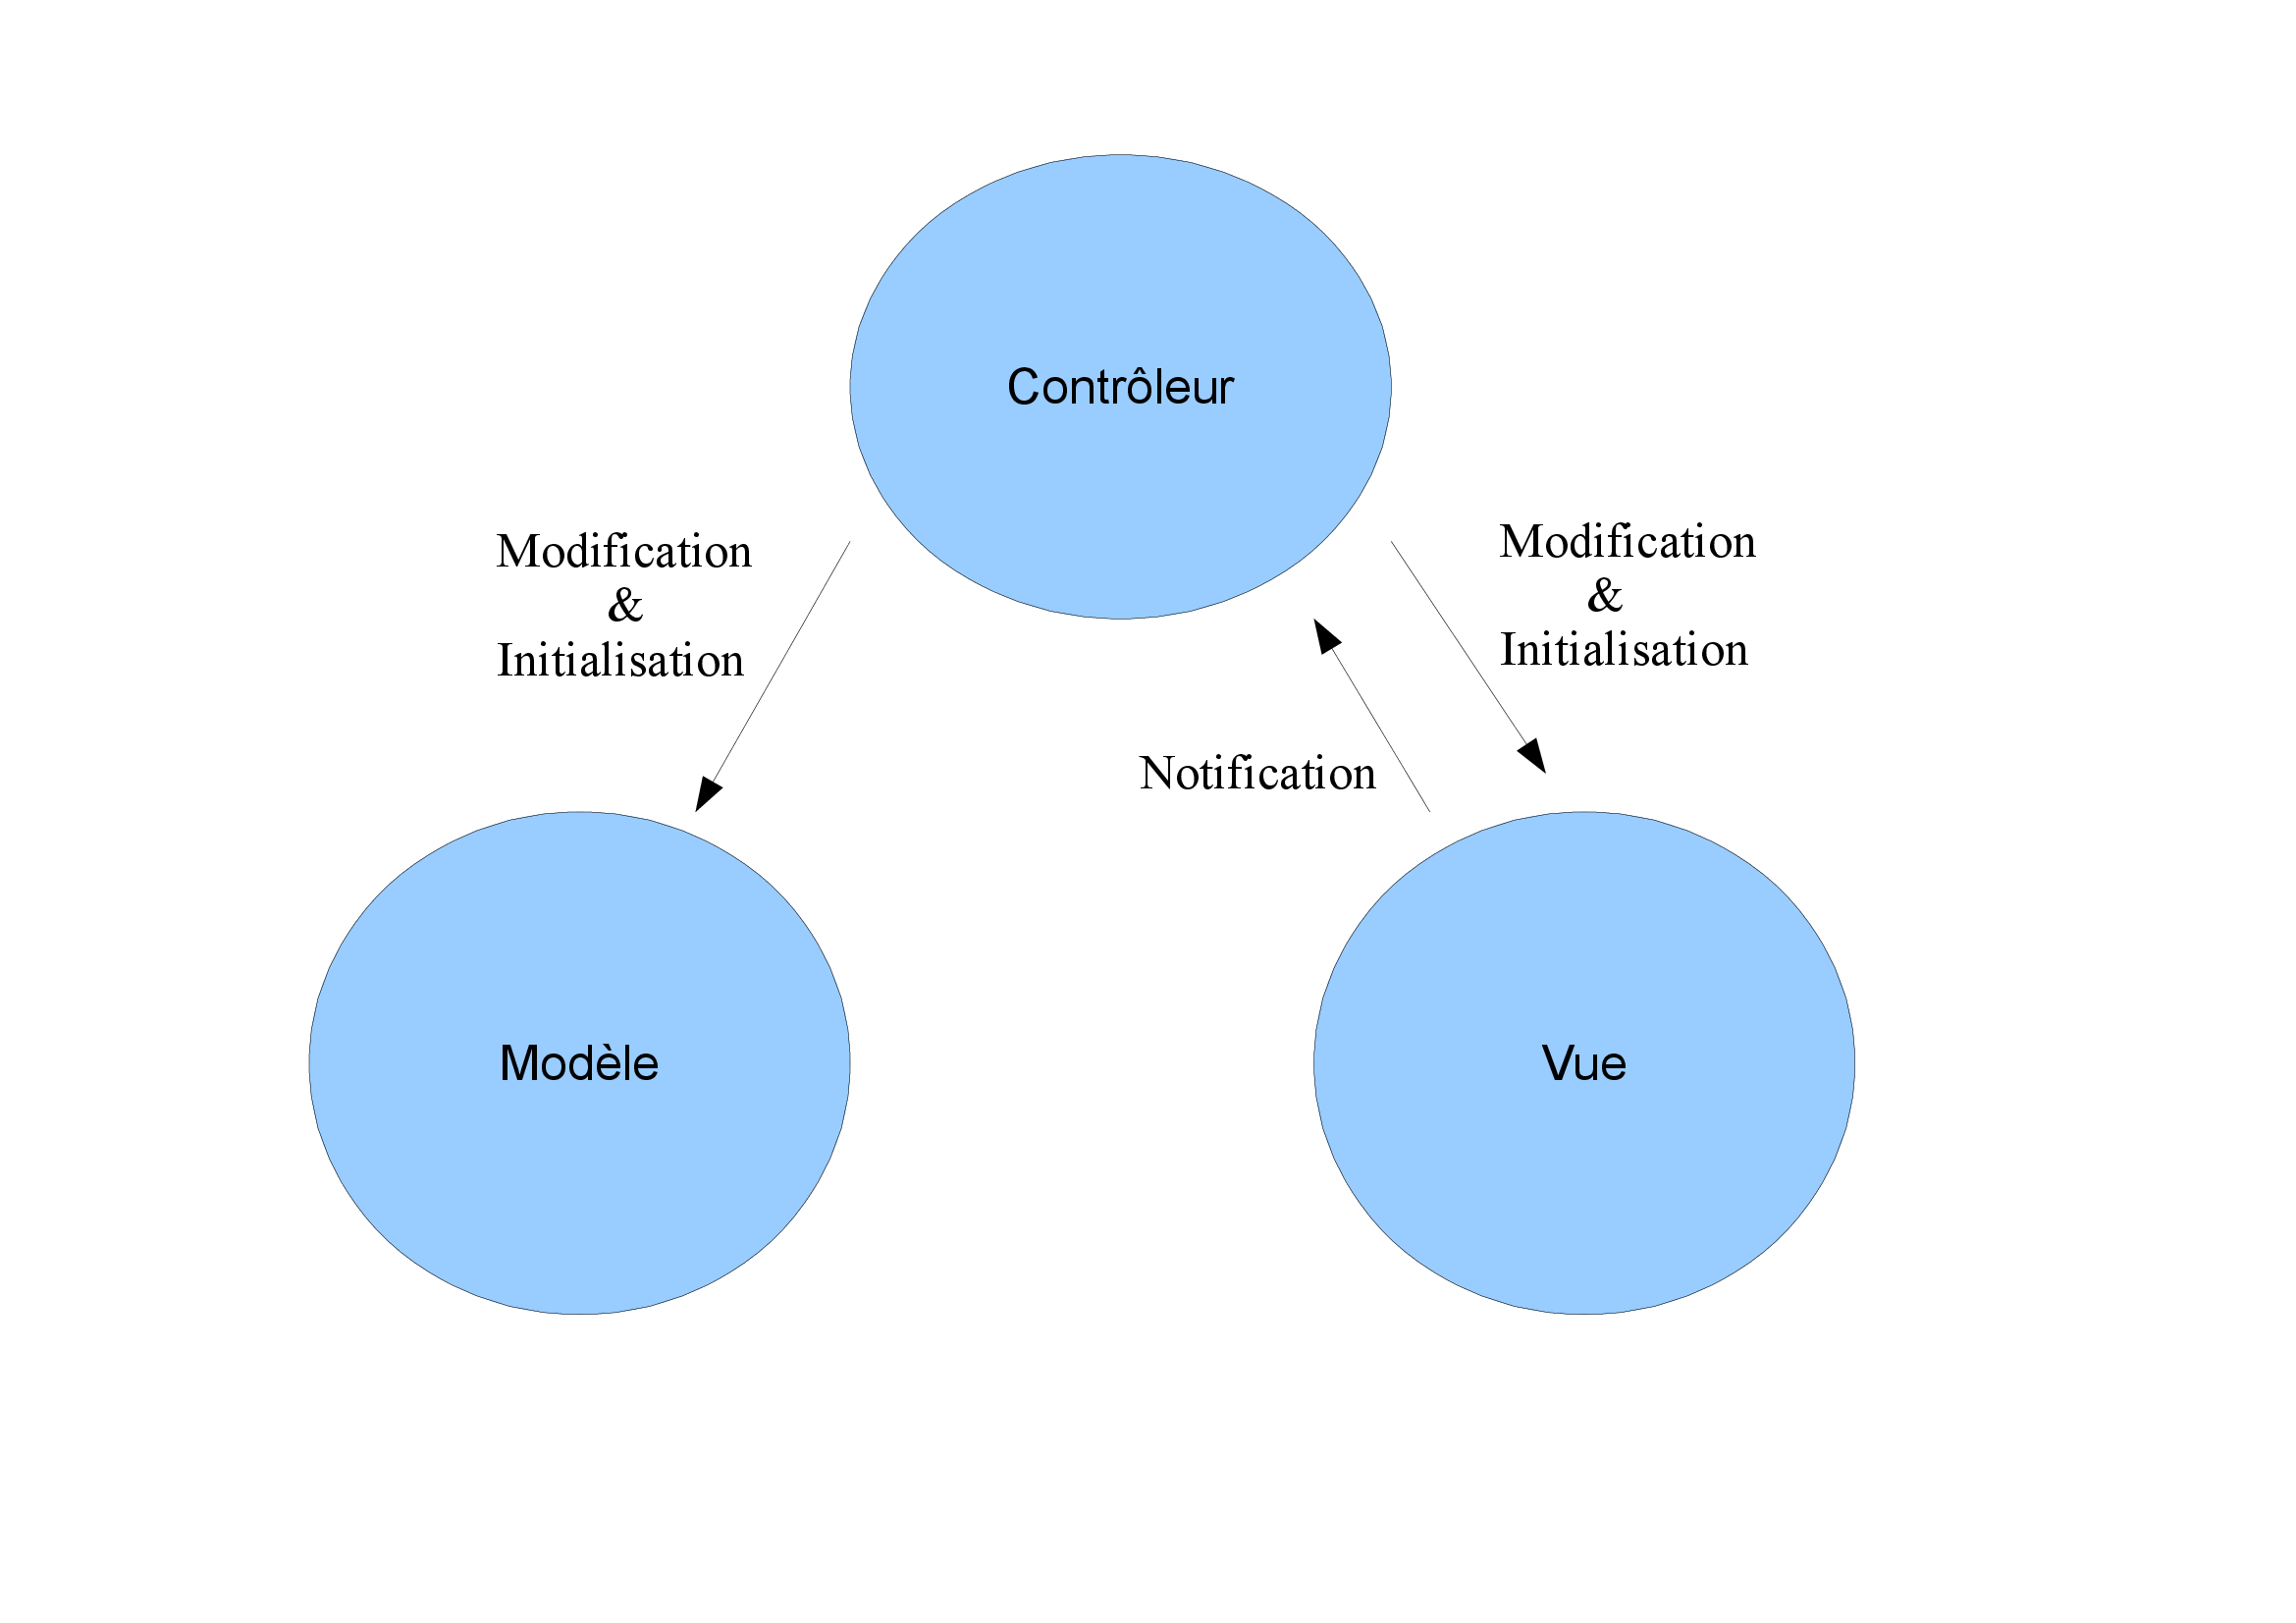
\includegraphics[scale=0.2]{img/mvc.png}

	Nous pouvons remarquer que la classe Controller est une «god class». En effet, tous les traitements effectués passent par cette classe. Lorsqu'on exécute le main, on crée un objet controller qui va générer le modèle et l'interface graphique. En effet, le constructeur de la classe Controller va appeler le constructeur de la classe Game ainsi que celui de la classe RasenderFrame. Ces deux classes correspondent respectivement à notre modèle et à notre vue.
	
	Ensuite, lorsque l'utilisateur va effectuer une action dans l'interface graphique, soit un click de la souris, soit l'appui sur un bouton utilisé dans notre jeu, le contrôleur va être avertit. À partir de là, le modèle va être mis à jour, puis l'interface graphique sera à son tour mise à jour.
	
	 Le fait que cette classe soit une «god class» n'est pas gênant pour ce logiciel. En effet, il n'y a pas de données critiques dans le jeu. Le seul risque est que la partie soit perdu, et que l'utilisateur doive en recommencer une depuis le début.

	
	\subsection{Exemple}
	
	Nous avons vu que le contrôleur initialise et modifie le modèle en fonction des événements que l'interface graphique lui envoie. 
Pour chaque bouton et chaque menu de notre fenêtre nous avons implémenté un «action listener» qui se trouve dans le contrôleur. De plus, pour les événements provenant du clavier ou de la souris, nous avons implémenté les interfaces «MouseListener» et «KeyListener».

	Par exemple, si l'on clique sur le robot rouge dans l'interface graphique, le contrôleur va recevoir cet événement et il va indiquer au modèle le changement à effectuer grâce à la méthode «setSelectedRobot(Robot r)». Ensuite, le contrôleur va avertir l'interface que le modèle a changé en appelant la fonction «refreshBoard». L'interface va donc se mettre à jour et afficher le bon plateau.
